\section{Combinatorial Search Approach}
\label{cha:combinatorialsearch}

This section introduces the idea behind the combinatorial search
approach, which is illustrated by Figure \ref{fig:cs_intro}. In this
figure, {\bf H} is the optimal decision hyperplane that separates the
two classes of the training dataset. {\bf H'} is another decision
hyperplane, which was obtained from {\bf H} by changing its direction
a little bit, so that it goes through the two points A and B nearest
to {\bf H}. Clearly, the loss value of any point in the training
dataset is unchanged when the decision hyperplane is moved from {\bf
  H} to {\bf H'}, because there is no point lying in between
them. Therefore, if {\bf H} is the optimal 0--1 loss solution, then so
is {\bf H'}, as they must have a same 0--1 loss value. This fact can
be exploited by assuming that the optimal decision hyperplane goes
through a certain number of points in the training dataset. For
example, in Figure \ref{fig:cs_intro} points are in $\R^2$, hence it
can be assumed that the optimal hyperplane goes through two points of
the training dataset, because two points defines a hyperplane (a line)
in $\R^2$. After that, the simple way to find the optimal solution is
to evaluate the 0--1 loss function of all $N(N-1)/2$ possible
hyperplanes and find the one that have minimum 0--1 loss value. In
general, if points in the training dataset are in $\R^D$, one needs
$D$ points to determine a hyperplane, which means the total number of
all possible hyperplanes to be assessed is ${N \choose D}$. It can be
seen, that by limiting the hyperplanes to those that go through the
given number of points of the training dataset, the search space has
been changed from an infinite continuous space to a finite discrete
one. Because of the fact that the search space is combinations of $D$
out of $N$ points, this approach is named combinatorial search for
0--1 loss optimization.

\begin{figure}[here]
\includegraphics[width=0.50\textwidth]{images/fig41_intro.eps}
\caption{ This plot illustrates the basic idea behind the
  combinatorial search approach. In the plot, {\bf H} is the optimal
  decision hyperplane to separate the two classes. {\bf H'} is
  obtained from {\bf H} by tuning its direction, so that it goes
  through the two nearest points A and B. Clearly, the 0--1 value
  stays unchanged if the decision hyperplane is moved from {\bf H} to
  {\bf H'}, because there are no points lying between them. Therefore,
  if {\bf H} is the optimal 0--1 loss solution, then so is {\bf H'},
  because their 0--1 loss value is the same. The combinatorial search
  approach exploits this fact to alter the search from an infinite
  continuous space to a finite discrete one by assuming that the
  optimal decision hyperplane goes through a certain number of points
  of the dataset.  }
\label{fig:cs_intro}
\end{figure}

To formally formulate the approach discussed above, it is necessary to
refer back to the definition of 0--1 loss optimization problem given
in Section \ref{sec:bgr.formulation} of Chapter \ref{cha:background},
wherein it was discussed that the best decision hyperplane is defined
by $\boldsymbol{{w^*}^Tx}=0$, where
$${\w}^* = \arg\min_{\w} L({\w}),$$ 
and 
$$L(\w) = \sum_{i=1}^N \mathbb{I} [t_i \w^T \xi \leq 0].$$ The given
problem definition used the homogeneous notation. In this chapter,
however, it is much more convenient to use the non--homogeneous
notation. In this case, the bias term $w_0$ is a separate scalar
variable, and $\xi, \w$ have the following format:
$$\xi =  (x_{i1}, x_{i2}, \dots, x_{iD})^T \in \R^{D}$$
$$\w = (w_1, \dots, w_D)^T \in \R^{D},$$
$$w_0 \in \R.$$ 
The 0--1 loss function is now equivalent to 
\begin{equation}\label{eq:loss}
L(w_0,\w) = \sum_{i=1}^N \mathbb{I} [w_0 + t_i (\w^T \xi) < 0].
\end{equation}
In this loss function definition, the non-strict inequality inside the
indicator function is replaced by a strict inequality for the
convenience of this approach. The only difference this makes is in the
way how to treat points lying directly on the decision hyperplane:
before these are deemed to be misclassified, now correctly
classified. As it is expected that there are none or only a few points
lying on the decision hyperplane, this difference is negligible.

A decision hyperplane that separates the two classes is now given by
$w_0 + \w^T\boldsymbol{x} = 0$, and the optimal solution $\w_{opt} =
(w_0^*, \w^*)$ consists of the bias and the weight vector that
minimizes the 0--1 loss function $L(w_0, \w)$ above. If the bias term
$w_0$ is zero, the decision hyperplane must go through the origin,
which is very rare in practice. Thus, it is reasonable to assume that
$w_0 \not= 0$. Then, if both $w_0$ and $w$ are scaled by $|w_0|$, the
solution is unchanged. To be more specific, there are two
cases. First, if $w_0>0$, then the loss function is:
\[ \begin{split}
L(w_0,\w) &= \sum_{i=1}^N \mathbb{I} [w_0 + t_i (\w^T \xi) < 0] \\
&=\sum_{i=1}^N \mathbb{I} [t_i (\frac{w_0}{|w_0|} + \frac{1}{|w_0|}\w^T \xi) < 0]  \\
&= \sum_{i=1}^N \mathbb{I} [t_i (1 + \w'^T \xi) < 0] \\
&= L(1, \w'),\\
\end{split} \]
where $\w'$ is defined as $\w' = \frac{1}{w_0}\w$. The equation of the
decision hyperplane is as follows:
\[ \begin{split} 
&w_0 + \w^T\boldsymbol{x} = 0 \\
\Leftrightarrow \quad
&\frac{w_0}{|w_0|} + \frac{1}{|w_0|} \w^T \boldsymbol{x}  = 0 \\ \Leftrightarrow \quad
&1 + \w'^T \boldsymbol{x} = 0
\end{split} \]
Second, if $w_0 < 0$, then $\w' = \frac{1}{w_0}\w = -\frac{1}{|w_0|}\w$, and the loss function is 
\[ \begin{split}
L(w_0,\w) &= \sum_{i=1}^N \mathbb{I} [w_0 + t_i (\w^T \xi) < 0] \\
&=\sum_{i=1}^N \mathbb{I} [t_i (\frac{w_0}{|w_0|} + \frac{1}{|w_0|}\w^T \xi) < 0]  \\
&= \sum_{i=1}^N \mathbb{I} [t_i (-1 - \w'^T \xi) < 0] 
= L(-1, -\w'),\\
\end{split} \]
and the equation of the decision hyperplane is 
\[ \begin{split} 
&w_0 + \w^T\boldsymbol{x} = 0 \\
\Leftrightarrow \quad
&\frac{w_0}{|w_0|} + \frac{1}{|w_0|} \w^T \boldsymbol{x}  = 0 \\ \Leftrightarrow \quad
&-1 - \w'^T \boldsymbol{x} = 0 \\
\Leftrightarrow \quad
&1 + \w'^T \boldsymbol{x} = 0
\end{split} \]
It can be seen, that the equation of the decision hyperplane ($1 +
\w'^T \boldsymbol{x} = 0$) is the same in both cases, and the loss
function is either $L(1, \w')$ or $L(-1, -\w')$, i.e., the bias term
is now a either $1$ or $-1$, not a variable like before. As shall be
seen next, this fact is critically important for the purpose of the
combinatorial search approach. The discussion at the beginning of this
section pointed out, that to find the optimal solution, it suffices to
check all hyperplanes that go through $D$ points of the training
dataset and find the one that has minimum 0--1 loss. So, assuming
$\boldsymbol{x_1}, \dots, \boldsymbol{x_D}$ are (any) $D$ distinct
data points from the training dataset, then for the combinatorial
search to work, the two following tasks must be solved:
\begin{itemize}
\item Find the weight vector $\w'=(w'_1, \dots, w'_D)^T$ of the
  decision hyperplane that goes through these $D$ selected points.
\item Calculate the 0--1 loss value corresponding to $\w'$.
\end{itemize}

For the first task, because the hyperplane goes through the given $D$
data points, at each point the hyperplane equation must be
satisfied. So,
$$ 1+ \w'^T\xi = 0, \quad\quad \text{for } i = 1, 2, \dots, D.$$
Now, let $A$ be a matrix, whose rows are formed by these points: 
$A =(\boldsymbol{x_1}\; \boldsymbol{x_2}\; \dots \; \boldsymbol{x_D})^T$,
then the weight vector $\w'$ must satisfy the following matrix equation 
\begin{equation}\label{eq:matrix}
\boldsymbol{1} + A \w' = 0 \Longrightarrow \w' = -A^{-1}\boldsymbol{1},
\end{equation}
where $\boldsymbol{1}$ is the unit vector in $\R^D$, because each row
of this matrix equation corresponds to an equation for one point given
above. Here, one sees that if the bias term $w_0$ was still present,
the above equation would be undetermined.

Now, with $\w'$ specified, the second task becomes easy, as the 0--1
loss value is obviously the smaller value of $L(1,\w')$ and $L(-1,
-\w')$. Thus, if $L(1,\w') \leq L(-1,-\w')$, the 0--1 loss value
corresponding to decision hyperplane $1+\w'^T\boldsymbol{x} = 0$ is
$L(1,\w')$, and the solution vector (including bias and weights) is
$(1, \w')$, otherwise, the 0--1 loss value is $L(-1,-\w')$, and the
solution vector is $(-1,-\w')$.

The above discussion represents all necessary knowledge for the
combinatorial search approach and it is now possible to build
algorithms based on the foundation presented here. Thus, the following
section outlines the first and simplest algorithm to illustrate the
combinatorial search concept. The section after that then proposes
more advanced algorithms, all of them utilizing the combinatorial
search approach.


%==========================
\subsection{Prioritized Combinatorial Search}
\label{sec:cs.prioritized}

\begin{figure}[here]
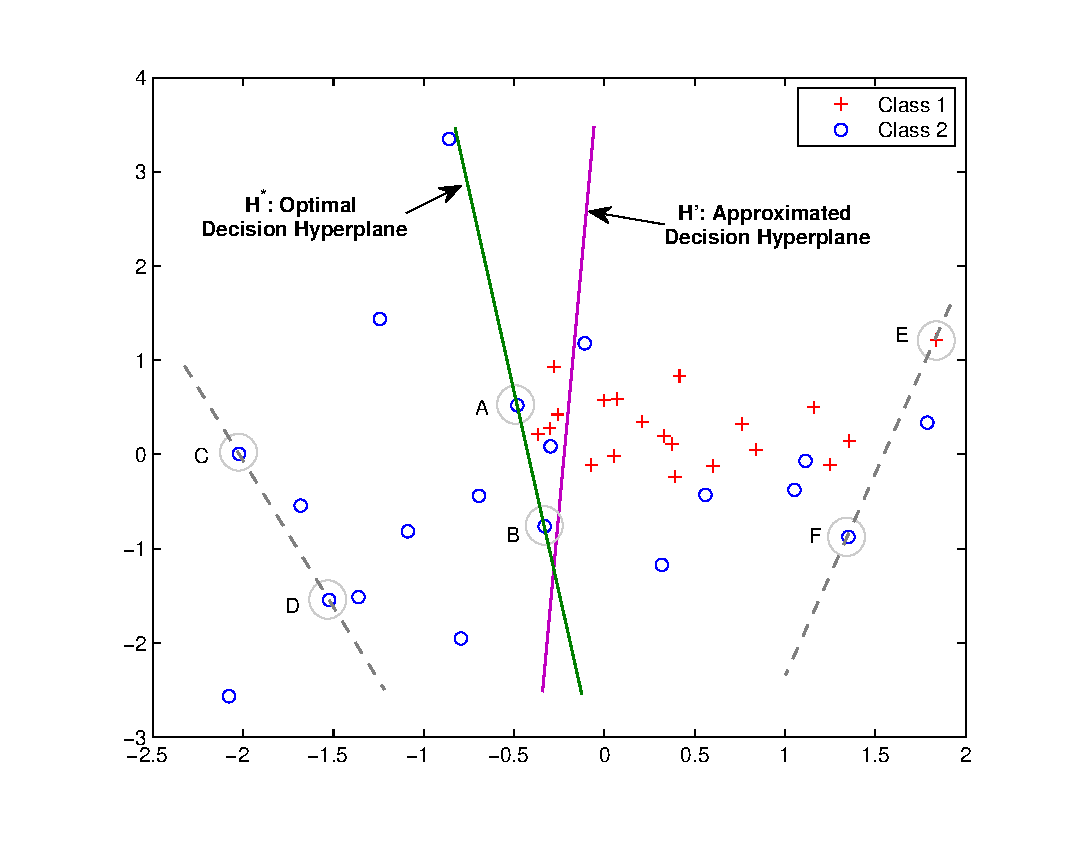
\includegraphics[width=0.50\textwidth]{images/fig42_nearfar.eps}
\caption{ This plot shows that combinations of points lying near to an
  initial approximated decision hyperplane are more likely to produce
  the optimal decision hyperplane (in the combinatorial search) than
  those far away. In the plot, H' is an initial approximated decision
  hyperplane (a line in this 2-D case) given by
  linear-SVM. H\textsuperscript{*} is the optimal decision hyperplane
  that going through points A and B near to H'. Clearly, any
  hyperplane going through any points far away from H', e.g., points
  C, D, E, F, is far from being optimal. Thus, the prioritized
  combinatorial search gives priority to combinations of points lying
  closer to the initial approximated decision hyperplane.  }
\label{fig:cs_nearfar}
\end{figure}

This subsection details the prioritized combinatorial search
strategy. This strategy exploits the fact, that combinations of data
points lying closer to an initial approximated decision hyperplane
(given by a fast classifier) are more likely to produce the optimal
hyperplane than combinations of points lying far away. This is
illustrated by Figure \ref{fig:cs_nearfar}, in which the optimal
decision hyperplane, H\textsuperscript{*}, given by the basic
combinatorial search algorithm, goes through points A, B, that lie
very near to the approximated decision hyperplane, H', given by linear
SVM method. On the contrary, any combination of (two) points that lie
far from H', for example, points C, D, E, F, would be likely bad
candidates for an optimal decision hyperplane.

Algorithm \ref{alg:cs.prioritized} captures the above idea by
considering combinations of $D$ points in the increasing order of
their distance to the approximated decision hyperplane, where distance
of a combination of points is the minimal distance from these points
to the approximated decision hyperplane. It turns out that the
incorporation of this prioritization into the basic combinatorial
search algorithm is easy, as instead of using the direct indexing,
e.g., 1 is the first point in the dataset, one can use indirect
indexing ordered by increasing distance, e.g., 1 is now the point with
the shortest distance, 2 is the point with second shortest distance,
etc. This indirect indexing list is realized in step 4 in Algorithm
\ref{alg:cs.prioritized}. As has been discussed before in Chapter
\ref{cha:branchandbound}, ordering by distance of points to a
hyperplane is the same as ordering by the absolute value of the dot
product of points with the weight vector of the hyperplane. Thus, step
4 uses the latter type of ordering, because the dot product is very
easy to calculate.

\begin{figure}
\caption{
Prioritized Combinatorial Search for 0--1 Loss Optimization. \\
\text{\hspace{2.1cm}} $Input$: Dataset of training data points $ \boldsymbol{X}$, their labelled class targets $\t$. \\
\text{\hspace{2.1cm}} $Output$: Optimal weight vector $\w^*$ minimizing 0--1 loss.
}
\label{alg:cs.prioritized}
\begin{algorithmic}[1]
\Function{Find-Optimal-01Loss-Solution}{$\X, \t$} \Comment{returns $\w^*$}
\State $\w^* \gets$ approximated weight vector given by a fast classifier
\State $loss_{min} \gets$ 0--1 loss implied by $\w^*$
\State $\boldsymbol{i} \gets$ indices of points ordered by $|{\w^*}^T\boldsymbol{x_k}|$, for $k=1, \dots, N$.
\State $\p \gets [1,2,\dots,D]$
\Comment{initialize the first combination of $D$ points}
\While{$\p \not= \emptyset$}
   \State $(\w,loss) \gets$ \Call{Get-Solution}{$\p$}
   \If {$loss < loss_{min}$}
      \State $(\w^*, loss_{min}) \gets (\w, loss)$
   \EndIf
   \State $\p \gets $ next combination of ${N \choose D}$, or $\emptyset$ if there is no more.
\EndWhile
\State \Return $\w^*$
\Statex
\Function{Get-Solution}{$\p$} \Comment{returns $(\w, loss)$ corresponding to $\p$}
   \State $A \gets (x_{i[p_1]} \, x_{i[p_2]} \, \dots \, x_{i[p_D]})^T$
   \State $\w' \gets -A^{-1} \boldsymbol{1}$
   \If {$L(1,\w') \leq L(-1,-\w')$}
      \State $\w \gets (1, \w')$
      \State $loss \gets L(1,\w')$
   \Else
      \State $\w \gets (-1, -\w')$
      \State $loss \gets L(-1,-\w')$
   \EndIf
   \State \Return {$(\w, loss)$}
\EndFunction
\Statex
\EndFunction
\end{algorithmic}
\end{figure}

Algorithm \ref{alg:cs.prioritized} is explained as follows. In step 2,
instead of being initialized to $\emptyset$ like in the basic
algorithm, $\w^*$ is now assigned to a weight vector approximated by a
fast classifier, e.g., linear SVM. Step 3 then assigns $loss_{min}$ to
the corresponding 0--1 loss value of the approximated weight vector
that was assigned to $\w^*$ in the previous step. The list of ordered
indices $\boldsymbol{i}$ is assigned in step 4 and allows referencing
to points in increasing distance to the approximated decision
hyperplane defined by $\w^*$. So, for example, $i[1]$ is the index of
the point with the shortest distance, $i[2]$ is the index of the point
with the second shortest distance, etc. Step 5 initializes $\p$ to the
first combination of $D$ points, just like in the basic
algorithm. However, as mentioned above, $\p$ now contains indirect
indices through $\boldsymbol{i}$. For example, $p_1 = 2$ would refers
to the point with the second shortest distance to the approximated
decision hyperplane, which is point $\boldsymbol{x}_{i[p_1]} =
\boldsymbol{x}_{i[2]}$. The while loop in steps 6 through 12 checks
all possible combinations of $\p$. Specifically, step 7 calls function
{\sc Get-Solution} to get the weights and loss value corresponding to
current combination $\p$ and assign them to $\w$ and $loss$. Step 8
checks, if this $loss$ is smaller than the current minimal value
$loss_{min}$, then the current minimal solution is updated in step
9. Step 11 generates the next combination of $D$ out of $N$ points and
assign to $\p$. If all possible combinations have been generated, $\p$
is assigned to $\emptyset$, so that the while loop is terminated, then
the solution $\w^*$ is returned in step 13.

In this algorithm, the process of getting solution from a combination
of $D$ points is separated into the function {\sc Get-Solution}, which
is given in steps 14 through 25. This function takes as input a list
of indirect indices of points (referenced by distance through
$\boldsymbol{i}$, so the true indices are $\boldsymbol{i[p]}$), and
return a weight vector $\w$ and 0--1 loss value $loss$ corresponding
to the hyperplane going through points
$\boldsymbol{i[p]}$. Specifically, step 15 assign the matrix $A$ with
row formed by points with indices $\boldsymbol{i[p]}$. Step 16 then
solves for $\w'$ in accordance with Equation \ref{eq:matrix}. Steps 17
through 23 calculates and compares the loss function in the two
possible cases as discussed in the foundation section. Thus, the loss
function is calculated by Equation \ref{eq:loss}, and values for the
weight vector $\w$ and the 0--1 loss value $loss$ are assigned
accordingly in steps 18-19, or 21-22.

Comparing to the basic algorithm, the prioritized combinatorial search
algorithm is initialized to an approximated solution, and allows to
find the optimal solution early in the search process. Thus, if the
algorithm's running time is limited, e.g., under two minutes, the
prioritized combinatorial search algorithm offers much better chance
of returning the optimal solution, and in the worst case, it would
return the approximated solution, which should be on average much more
useful than the result returned by the basic algorithm after having to
exit due to reaching the time limit. It, however, can be seen that the
two algorithms have the same complexity, and there's no gain for the
prioritized combinatorial search algorithm if the time limit is not
used. A possible way to achieve a significant reduction in the
complexity of combinatorial search is by relaxing the optimization
problem to approximate solution instead of finding optimal one. This
topic shall be discussed in the next subsection

%==========================
\subsubsection{Combinatorial Search Approximation}
\label{sec:cs.greedy}

So far, algorithms in this chapter haven't broken the curse of the ${N
  \choose D}$ complexity of the combinatorial search approach (anytime
property apart). This subsection examines an approximation algorithm
that offers significant lower complexity, while returning good
approximate solution close to the optimal one.

\begin{figure}
\caption{
Combinatorial Search Approximation for 0--1 Loss Optimization. \\
\text{\hspace{2.1cm}} $Input$: Dataset of training data points $ \boldsymbol{X}$, their labelled class targets $\t$. \\
\text{\hspace{2.1cm}} $Output$: Optimal weight vector $\w^*$ minimizing 0--1 loss.
}
\label{alg:cs.approximation}
\begin{algorithmic}[1]
\Function{Approximate-01Loss-Solution}{$\X, \t$} \Comment{returns $\w^*$}
\State $\w^* \gets$ approximated weight vector given by a fast classifier
\State $\boldsymbol{i} \gets$ indices of points ordered by $|{\w^*}^T\boldsymbol{x_k}|$, for $k=1, \dots, N$.
\State $(\p, \w^*, loss_{min}) \gets$ \Call{Get-Best-Initial-Solution}{$30$}
\Loop
   \For {$k=1$ to $N$}
      \If {$k \not\in \p$}
         \For {j=1 to D} 
            \State $\p' \gets \p$
            \State $p'_j \gets k$
            \Comment{replace $j-$th component by $k$}
            \State $(\w, loss) \gets$ \Call{Get-Solution}{$\p'$}
            \If {$loss < loss_{min}$}
               \State $(\p, \w^*, loss_{min}) \gets (\p', \w, loss)$
               \State {\bf go back to step 5}
            \EndIf
         \EndFor
      \EndIf
   \EndFor
   \State \Return $\w^*$
 \EndLoop
\Statex
\Function{Get-Best-Initial-Solution}{$N'$} \Comment{returns $(\p, \w, loss)$}
   \State $loss \gets +\infty$
   \State $\p_t \gets [1,2,\dots,D]$
   \Comment{initialize the first combination of $D$ points}
   \While{$\p_t \not= \emptyset$}
      \State $(\w_t, loss_t) \gets$ \Call{Get-Solution}{$\p_t$}
      \If {$loss_t < loss$}
         \State $(\p, \w, loss) \gets (\p_t, \w_t, loss_t)$
      \EndIf
      \State $\p_t \gets $ next combination of ${N' \choose D}$, or $\emptyset$ if there is no more.
   \EndWhile
   \State \Return $(\p, \w, loss)$
\EndFunction
\Statex
\EndFunction
\end{algorithmic}
\end{figure}

Approximation is relaxation to the 0--1 loss optimization problem, so
that instead of finding the optimal solution, the task is ``relaxed''
to approximate it. The idea behind the combinatorial search
approximation is to start from an initial combination of $D$ points
and gradually improve it until no further improvement is possible. To
be more specific, the algorithm starts from an initial ``best''
combination of $D$ points near to an approximated decision hyperplane
given by some fast classifier, then each time it swaps two points
$(\boldsymbol{x_k, x_j})$ in/out of the current combination, where
$\boldsymbol{x_k}$ is not in the current combination, but
$\boldsymbol{x_j}$ is, and by putting $\boldsymbol{x_k}$ into and
remove $\boldsymbol{x_j}$ out of the current combination, the 0--1
loss value corresponding to the new combination is reduced. The
algorithm stops when it can not find any more points to swap. This
algorithm is detailed in Algorithm \ref{alg:cs.approximation}. It may
sound complicated, but is rather simple, and an explanation is given
below.


\begin{figure}[here]
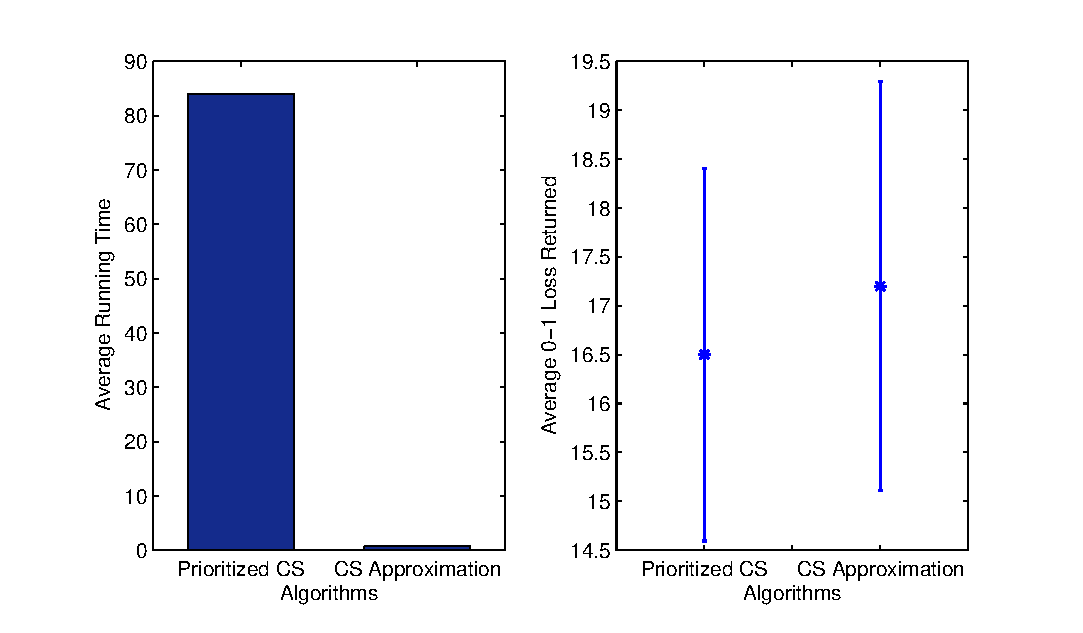
\includegraphics[width=0.50\textwidth]{images/fig43_approx.eps}
\caption{ This plot shows the improvements of the approximation
  algorithm over the prioritized combinatorial search. 20 tests of
  size $N=60$ and dimension $D=4$ have been generated with different
  0--1 loss values from 14 to 22. The plot on the left shows the
  average running time of each algorithm. This number with one
  standard deviation for the approximation algorithm was $0.73 \pm
  0.03$, whereas it was $83.93 \pm 1.32$ for the prioritized
  combinatorial search algorithm. The plot on the right shows the mean
  value of 0--1 loss returned by each algorithm, including the error
  bar of one standard deviation. This number for the prioritized
  combinatorial search was $16.50\pm 1.91$, and $17.20 \pm 2.09$ for
  the approximation algorithm. As can be seen, the gain in performance
  of approximation is significant, while the result is obviously very
  close to the optimal solution. This is also evidenced by Figure
  \ref{fig:cs_approxlosses}, a continuation of this figure.  }
\label{fig:cs_approx}
\end{figure}

\begin{figure}[here]
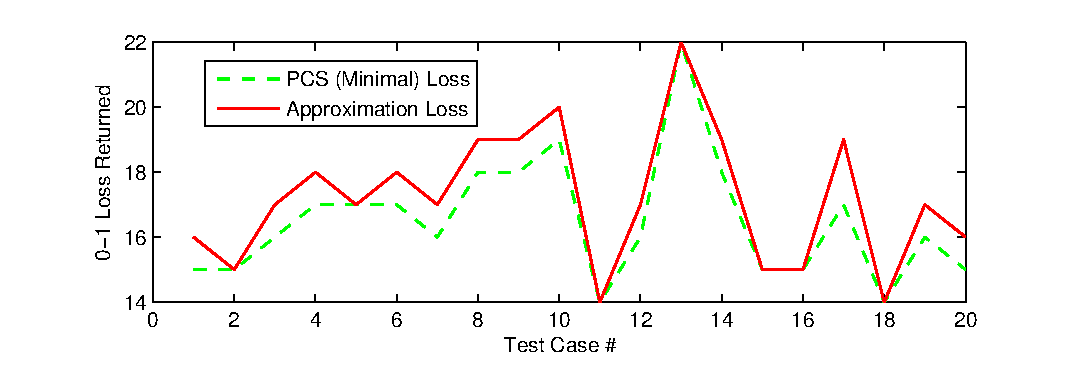
\includegraphics[width=0.50\textwidth]{images/fig44_approxlosses.eps}
\caption{ This plot is a continuation of Figure \ref{fig:cs_approx}
  and shows the optimal 0--1 loss returned by the prioritized
  combinatorial search (PCS) versus value returned by the
  approximation algorithm for each of the 20 tests. It can be seen,
  that the approximation follows the optimal value very closely. In
  fact, the difference between loss values returned by the two
  algorithms was $0.70 \pm 0.57$.  }
\label{fig:cs_approxlosses}
\end{figure}

{\bf NOTE: Fast and close to optimal.}

%=================================================
\subsection{Complexity Analysis of Combinatorial Search}
\label{sec:cs.performance}

The performance of the combinatorial search algorithms introduced in
this chapter are much easier to analyze comparing to the performance
of branch and bound algorithms studied in Chapter
\ref{cha:branchandbound}. In fact, the complexity of all algorithms in
this chapter can be examined analytically and exact formulas for
complexity can be given directly, as shown in the rest of this
section.

%========================
\subsubsection{Complexity of Basic Combinatorial Search}

For the complexity of the Algorithm \ref{alg:cs.basic}, the while loop
in steps 5 to 17 loops exactly ${N \choose D}$ times, as that many
combinations of $D$ out of $N$ points are generated in step 16. There
are only a few complexity significant steps inside the body of this
loop as follows. Step 7 solves the matrix equation of size $D$, which
is $\approx O(D^{2.4})$ by using Coppersmith--Winograd algorithm
\cite{Coppersmith}. The calculation of 0--1 loss function $L(1,\w')$
and $L(-1,-\w')$ in steps 8-15 clearly takes times $O(ND)$. The
algorithm to generate combinations of ${N \choose D}$ can be easily
implemented in an incremental way with cost $O(D)$. Thus, assuming $D
<< N$, which means $O(D^{2.4}) < O(ND)$, then the exact complexity of
Algorithm \ref{alg:cs.basic} is $O\{ ND{N \choose D} \}$. For smaller
dimensionality $D$, this is equivalent to $O(N^{D+1})$, e.g., for
$D=3$, the complexity is $N^4$. For higher dimensionality, however,
the complexity is huge.

%========================
\subsubsection{Complexity of Prioritized Combinatorial Search}

It can be seen, that Algorithm \ref{alg:cs.prioritized} must have the
same complexity as that of Algorithm \ref{alg:cs.basic}, because they
share similar structure, with the only difference is in building the
list $\boldsymbol{i}$ of indices ordered by distance to the
approximated decision hyperplane in step 4, which takes $O(N \log N)$,
less than the complexity of $O\{ ND{N \choose D} \}$ of the while
loop. So overall complexity of Algorithm \ref{alg:cs.prioritized} is
$O\{ ND{N \choose D} \}$. And its advantage over the basic algorithm
lies in the $anytime$ design, and the ability to find optimal solution
earlier in the search process.

%========================
\subsubsection{Complexity of Combinatorial Search Approximation}

The approximation algorithm outlined in Algorithm
\ref{alg:cs.approximation} has two distinct parts. The first part is
the call to the function {\sc Get-Best-Initial-Solution} to determine
the best solution of a small number of points nearest to an initial
approximated decision hyperplane. This part is basically the
application of Algorithm \ref{alg:cs.prioritized} on a limited scale
of $N'$ points, so the complexity is $O\{ N'D{N' \choose D} \}$. The
second part consists of the loop at step 5, which in each repeat
reduces $loss_{min}$ by at least one unit. The loss value is bounded
by the number of data points, $N$. So the loop at step 5 repeats
maximally $N$ times. The two for loops at steps 6 and 8 clearly repeat
maximally $ND$ times. Steps 9 to 15 is the body of these for loops,
and have combined complexity $O(ND)$, because the most significant
step is the calculation of the 0--1 loss function, which takes $O(ND)$
time. So, the for loops in steps 6 to 18 takes $O(N^2D^2)$ time,
hence, the second part of the algorithm takes time $O(N^3D^2)$. It has
been discussed, that the parameter $N'$ of the {\sc
  Get-Best-Initial-Solution} should be small enough, such that this
function does not take a long time to compute. Thus, it can be assumed
that $O\{ N'D{N' \choose D} \} < O(N^3D^2)$. So, all together, the
overall complexity of Algorithm \ref{alg:cs.approximation} is
$O(N^3D^2)$. Note that this is the worst case scenario. Clearly, the
average performance is much better, because the loops are broken
immediately when a better solution is found.

In Figure \ref{fig:cs_approx} presented in previous section, the
performance of these algorithms were compared (Algorithm
\ref{alg:cs.basic} and Algorithm \ref{alg:cs.prioritized} should have
similar performance), and the average running time of the
approximation algorithm is well under a second for problem size of
$N=60, D=4$, which is about 100 times smaller than the running time of
84 seconds of the prioritized combinatorial algorithm.
